
\newpage
\null

\begin{center}
    \Huge{\textbf{\underline{Chapter 2: Lexical Analysis}}}
\end{center}

\setcounter{section}{0}

\vspace{0.35cm}


\section{Lexical Analysis}

\begin{prettyBox}{Lexical Analysis}{myblue}
The first step of compilation takes the source code as input,  
representing a sequence of characters separated or not by  
spaces and new lines. It consists of:  

\begin{itemize}
    \item Fetching all lexical entities (tokens) and verifying  
        whether they are part of the language. The tokens are then  
        classified as constants, identifiers, keywords, or separators.  
    \item Removing all extra spaces and comments.  
    \item Producing a chaine of code (sequence of tokens) that will be used in syntactic analysis.  
    \item Initializing the \textbf{symbol table} (dictionary) by inserting  
        the retrieved tokens and their corresponding codes after verification (tokens must be unique (no repetition)). The symbol table will be updated  
        as we progress through the next compilation steps.  
\end{itemize}
\end{prettyBox}

\vspace{0.75cm}
\section{Notes}

\begin{prettyBox}{Optimization}{red}

\begin{itemize}
    \item In real-life implementations, the symbol table is often divided into sub-tables  
        based on token types improving search speed  
        and optimizes memory usage.  
    \item We can also prefill the table of keywords and separators since they are known
in advance. This simplifies the automaton, as it no longer needs states to recognize keywords and separators , it can directly compare tokens to the prefilled tables.
\end{itemize}
\end{prettyBox}

\vspace{0.5cm}



\begin{prettyBox}{Reserved Words \& Keywords}{red}
\begin{itemize}
\item \textbf{Keywords :} are special tokens in a programming language that have predefined semantic meanings, such as data types, control flow structures, or loop constructs (e.g., `if`, `while`, `int`, `return`). These words are integral to the syntax of the language.
\item \textbf{Reserved words :} are tokens that cannot be used as identifiers (like variable or function names) because they are reserved for the language's future use or for language-specific functionality.
\item In most compilers, \textbf{all keywords are reserved words}. However, some non-standard or unconventional compilers may allow certain reserved words to be used as identifiers. For example, in these compilers, you might be able to write code like `int if = 5;`, which is not allowed in standard compilers.
\end{itemize}
\end{prettyBox}

\newpage
\null


\begin{prettyBox}{Two Schools of Thought}{red}
Imagine encountering \(><\):  
\begin{itemize}
    \item \textbf{Method 1}: Considers \(><\) as a single token and checks it against the prefilled separator table. Since no match is found, it is classified as a lexical error.  
    \item \textbf{Method 2}: Recognizes \(>\) and \(<\) as separate, valid tokens but considers their order incorrect, making it a syntactic error. This approach is more practical , and used
        in most compilers.  
\end{itemize}
\end{prettyBox}

\vspace{0.5cm}
\section{Implementation of Lexical Analysis}  
\begin{prettyBox}{Implementation}{myblue}  
Lexical analysis utilizes a finite deterministic automaton to break the source code into  
lexical entities (tokens) and verify their validity within the language.  
To implement the automaton, we need to:  
\begin{itemize}  
    \item Choose a suitable data structure to represent the automaton in memory.  
    \item Develop an algorithm for tokenizing the source code and validating tokens.  
\end{itemize}  
\end{prettyBox}  

\vspace{0.5cm}

\subsection{Representation of Automaton}

\begin{prettyBox}{Representation}{myblue}
\begin{itemize}
    \item The automaton will be represented by a transition matrix, where each row corresponds to a state, and each column represents a letter.
    \item An array will be used to store the final states.
    \item A constant will define the initial state.
\end{itemize}
\end{prettyBox}

\vspace{0.75cm}

\begin{prettyBox}{Reminder}{red}
    \begin{itemize}
        \item \textbf{Deterministic:} At most one transition is possible from state \( e_0 \) to \( e_1 \) for a given letter \( l_0 \).  
        \item \textbf{Finite:} The automaton has a limited number of states and transitions.  
        \item \textbf{Token Acceptance:} A token is considered valid if the automaton processes it without encountering a dead end (no blockage) and reaches a final state.  
    \end{itemize}
\end{prettyBox}

\newpage
\null

\textbf{\underline{Example}}\\[0.5cm]
L = \{ u \(\in \{0,1\}^{*}\) / \(|\text{W}|_{0}\) \(\equiv\) 0[2]\}

\vspace{0.15cm}

\begin{center}
    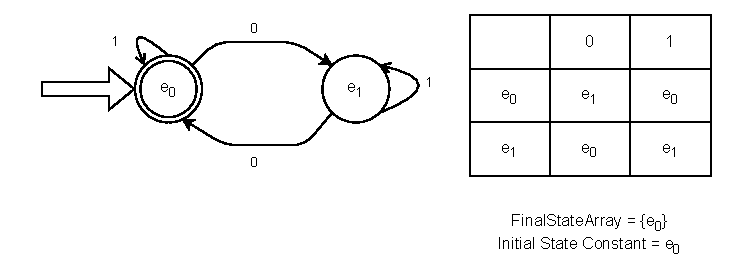
\includegraphics[width=0.8\textwidth]{Chapters/Examples/Lexi/ex1.drawio.pdf}
\end{center}

\vspace{0.4cm}
\textbf{\underline{Execution Of The Automata For The Word 1011}}\\[0.25cm]

\begin{center}
    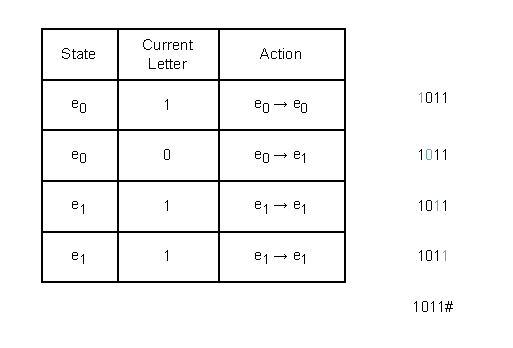
\includegraphics[width=0.8\textwidth]{Chapters/Examples/Lexi/ex1.1.drawio.pdf}
\end{center}

\newpage
\null

\begin{prettyBox}{Conclusion}{myblue}
Even though there is no blockage when the automaton reads \(1011\),  
it does not reach a final state in the end. Since \( e_1 \notin \) FinalStateArray, we conclude:  
\[ \boxed{1011 \notin \text{L}} \]
\end{prettyBox}

\vspace{0.5cm}

\begin{prettyBox}{Note}{red}
The symbol \# is used to mark the end of each token.
\end{prettyBox}

\vspace{0.5cm}

\subsection{Algorithm of Reconnaissance}
\begin{prettyBox}{Algorithm}{myblue}
The algorithm utilizes a finite deterministic automaton represented as a 
transition matrix. A token is recognized by the automaton if and only if 
it reaches '\#' in the token's terms and a final state in the automaton.\\[0.15cm]
We will first present the reconnaissance algorithm for a single token, followed by its application to an entire source code.
\end{prettyBox}

\vspace{1cm}

\subsubsection{Variables \& Predefined Functions}
\begin{prettyBox}{Notation}{myblue}
\begin{itemize}
    \item \textbf{Entity}: Lexical entity (token).
    \item \textbf{t\(_c\)}: Current term of the token.
    \item \textbf{t\(_s\)}: Next term of the token.
    \item \textbf{F}: Array of final states.
    \item \textbf{E\(_c\)}: Current state of the automaton.
    \item \textbf{M}: Transition matrix.
    \item \textbf{Lire(Entity)}: Reads a lexical entity from the source code, stores it in the \textbf{Entity} 
    variable, and appends '\#' at the end.
    \item \textbf{Saut\_Blanc()}: Skips whitespace, including tabulations and newline characters and comments.
\end{itemize}
\end{prettyBox}

\newpage

\begin{algorithm}
\caption{Algorithm Reconnaissance Of Single Token}
\begin{algorithmic}[1]
\debut
\lire{Entity}   \com{1.95}{Reads token}
\State t\(_{c}\) \affect Entity[0]; \com{1.6}{Initializ with 1st character} 
\State E\(_{c}\) \affect Initial State; \com{1}{Intialize with initial state}
\vspace{0.5em}
\While{( E\(_{c}\)\pase \vide\et t\(_c\) \pase \str{\#} )} \com{0.5}{Loop as long as there is no blockage and not all character of the token have been analyzed}
\vspace{0.25em}
\State E\(_c\) \affect M[E\(_c\),t\(_c\)]; \com{1}{Gets next state}
\State t\(_c\) \affect t\(_s\);            \com{2.1}{Gets next character of the token}
\vspace{0.25em}
\EndWhile

\vspace{0.5em}

\If{( E\(_c\)\pase \vide )} \com{1}{Check if there is a blockage}

\vspace{0.25em}
\pr{Error the lexical entity isn't regonised by the automaton because blockage happened}

\vspace{0.25em}
\ElsIf {( E\(_c\) \nin F )} \com{1}{Check if automaton reaches a final state}

\vspace{0.25em}
\pr{Error the lexical entity isn't regonised by the automaton because it didn't reach a final state}

\vspace{0.25em}
\Else  \com{1}{Token is regonized}

\vspace{0.25em}
\State Codify the lexical entity and put it in the symbole table.

\vspace{0.25em}
\EndIf
\fin
\end{algorithmic}
\end{algorithm}

\vspace{1cm}
\begin{algorithm}
\caption{Algorithm Reconnaissance Of All Tokens}
\begin{algorithmic}[1]
\debut
\jmp \com{1}{Ignores spaces , newlines and comments before reading the token}

\vspace{0.5em}
\While{( \n EOF )} \com{1}{Loop as long as we didn't reach EOF(End Of File)}
\vspace{0.25em}
\lire{Entity}      \com{1}{Reads token}

\vspace{0.15em}
\State Rest Of The Algorithm Of Reconnaissance Of Single Token
\vspace{0.15em}
\jmp
\vspace{0.25em}
\EndWhile
\fin
\end{algorithmic}
\end{algorithm}

\newpage

\textbf{\underline{Example}} \\[0.15cm]
Language of binary code with no successive 0s:
\begin{itemize}
    \item Create the transition matrix
    \item Analyze `101\#`
\end{itemize}

\begin{center}
    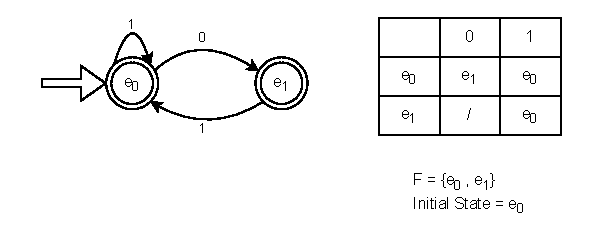
\includegraphics[width=0.8\textwidth]{Chapters/Examples/exalgo.drawio.pdf}
\end{center}

\vspace{0.5cm}

\begin{center}
    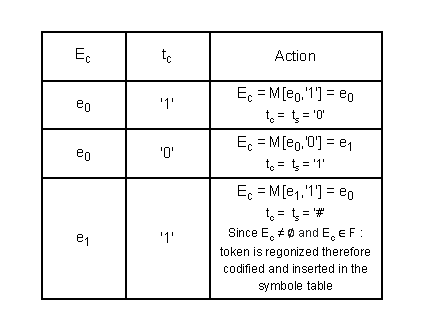
\includegraphics[height=0.5\textheight]{Chapters/Examples/exec.drawio.pdf}
\end{center}


